\documentclass[cn,11pt,chinese]{elegantbook}

\title{现代仪器分析复习提纲}
\subtitle{Review Outline on Contemporary Instrumental Analysis}

\author{化生81 期末资料编写组}
\institute{化生试验班81}
\date{\zhtoday}
\version{1.0}
%\bioinfo{自定义}{信息}

%\extrainfo{温柔正确的人总是难以生存,因为这世界既不温柔,也不正确。—— 比企谷八幡}

\logo{xjtu.png}
\cover{plastic.png}
% 本文档命令
\usepackage{array}
\newcommand{\ccr}[1]{\makecell{{\color{#1}\rule{1cm}{1cm}}}}

% 自定义设置
\usepackage[version=4]{mhchem}

%自定义微分号
\newcommand{\di}[1]{\mathrm{d}#1}
\newcommand{\p}[2]{\dfrac{\partial #1}{\partial #2}}
\newcommand{\pp}[2]{\dfrac{\partial ^2 #1}{\partial #2 ^2}}
\newcommand{\dy}[2]{\dfrac{\di{#1}}{\di{#2}}}
\newcommand{\ddy}[2]{\dfrac{\mathrm{d} ^2 #1}{\mathrm{d} #2 ^2}}

\newcommand{\tabincell}[2]{\begin{tabular}{@{}#1@{}}#2\end{tabular}}%单元格内强制换行

\usepackage{graphicx}   % 导入图片
\usepackage{subfigure}  % 并排子图


%模板中添加了
%\newtcbtheorem

% 本文档命令
\usepackage{array}
\newcommand{\ccr}[1]{\makecell{{\color{#1}\rule{1cm}{1cm}}}}

\begin{document}

\maketitle
\frontmatter

\chapter*{编写说明}
\markboth{Introduction}{编写说明}

随着科技的进步,各种仪器逐渐成为科学研究中必不可少的工具。为了探寻微观世界的奥秘,精确探测物质结构、含量、分布,获取有关研究体系的信息,研究人员都必须借助仪器这只“眼睛”。正是因为有了更精良的仪器,很多领域的科学问题才得以逐渐被科学家解决。可以说,没有仪器,就没有如今的科学成果。

《现代仪器分析》是化生试验班的一门专业核心课程,占2学分,讲授共32学时,由生命学院开设。课程涉及的主要学科是\textbf{分析化学},旨在帮助同学们掌握化学和生物研究中常用也是基础的仪器的原理、结构、适用范围等,为将来进入实验室进行实际操作打下理论基础。
这些分析手段的主要目的有二:检测(定性、定量)和分离,几乎每一章节在两方面都有所涉及。不过,各章节之间并没有紧密的联系,几乎是可以独立进行学习的。这些检测手段相互补充,共同构成了这门课的知识体系。

本课程的期末考试占总成绩的$70\%$,所以期末综合复习显得比较重要。为了明确课程要求同学掌握的内容,授课教师提供了一份提纲,为同学指明了需要复习的重点内容。为了方便同学们复习,化生81班班委组织了一些成绩优秀的同学梳理了提纲涉及的具体知识点,并用\LaTeX 整理成书。课程内容主要分为八章,分别列于下方框中。
\begin{tcolorbox}[title={\bfseries 编写组成员}]
	\ding{228} 张天翊:第一章\hspace{1em}\textbf{色谱}\\
	\ding{228} 王炜喆:第二章\hspace{1em}\textbf{质谱}\\
	\ding{228} 何琦璟;第三章\hspace{1em}\textbf{紫外-可见吸收光谱}\\
	\ding{228} 张宇博:第四章\hspace{1em}\textbf{分子发光分析}\\
	\ding{228} 郭骐瑞:第五章\hspace{1em}\textbf{红外光谱和拉曼光谱}\\
	\ding{228} 程肖然:第六章\hspace{1em}\textbf{核磁共振波谱}\\
	\ding{228} 高旭帆:第七章\hspace{1em}\textbf{电化学分析}\\
	\ding{228} 刘祎宁:第八章\hspace{1em}\textbf{原子光谱}\\
	\ding{228} 高旭帆、郭骐瑞:\textbf{排版、设计、整理}
\end{tcolorbox}
在此要对组织、编写和排版人员表示衷心的感谢!

在这份提纲中,有大量知识点需要记忆,希望同学们根据提纲有侧重点地复习。同时,这是化生试验班的第一份集体复习资料,各位编写者、排版者的风格可能有一定差异,内容、细节也存在可能的疏漏,必要时读者可以查阅课本、课件等其他资料。欢迎大家对这份提纲提出建议,也更希望大家多多支持我们的作品!

最后,我们希望这份提纲能帮助同学们取得一个理想的成绩!

\vskip 1.5cm

\begin{flushright}
	化生81 期末资料编写组\\
	2020\ 年\ 5\ 月\ 17\ 日
\end{flushright}

\tableofcontents
%\listofchanges

\mainmatter


\chapter*{排版格式介绍}
\begin{introduction}
	\item 概念及定义
	\item 公式
	\item 笔记
	\item 例子
\end{introduction}

以上是内容提要,大致概括本章的考点。

\section{几种环境}
我们将把每一个大问题作为一个section。

排版过程中的定义我们使用如下格式:

\begin{definition*}{概念及定义}{definition}
	
\end{definition*}

一些比较重要的公式我们使用如下格式
\begin{theorem*}{公式/定理}{theo}
	
\end{theorem*}

或者直接使用没有定理环境的
\begin{emptytcb*}{荧光的原理}{}
	受光激发的分子从第一激发单重态的最低振动能级回到基态所发出的辐射。
\end{emptytcb*}

因为我们保留了老师提供的提纲的顺序,我们并没有编号,否则会有点乱。

\note 需要补充、解释的我们加在这里

\begin{example}
	举例我们放在这里
\end{example}

\chapter{分子发光分析}

\begin{introduction}
	\item 分子发光及其产生原理(理解)
	\item 荧光定量分析有关概念(熟悉)
	\item 荧光分光光度计(熟悉)
\end{introduction}


%设计方案:
%1.定义、概念、原理,做个环境
%2.公式、符号说明环境
%3.步骤、结构、小点:列表
%4.对比:表格
某些物质的分子吸收一定能量跃迁到较高的电子激发态后,在返回电子基态的过程中伴随有光辐射,这种现象称为分子发光
分子发光具有如下特点:
\begin{itemize}
	\item 灵敏度高,检测下限比分光光度法低2-4个数量级
	\item 选择性比分光光度法好
	\item 分子发光分析体系应用有限,不如分光光度法广泛
\end{itemize}
\section{分子发光及其产生原理}

\begin{definition*}{荧光的原理}
	受光激发的分子从第一激发单重态的最低振动能级回到基态所发出的辐射。寿命为$10^{-8} \sim 10^{-11}\mathrm{s}$。由于是相同多重态之间的跃迁,几率较大,速度快,速率常数$k_f$为$10^{6}\sim 10^{9} \mathrm{s}^{-1}$。
\end{definition*}
荧光光谱形状的决定因素:
\begin{itemize}
	\item 固定激发光波长的荧光发射光谱(荧光光谱),测定某波长处的荧光发射强度与发射波长有关;
	\item 斯托克斯位移(激发光谱和发射光谱之间波长差值):振动、热辐射会使分子失去能量,即激光与发射荧光间的能量损失;
	\item 荧光发射光谱与激发波长无关
	\item 吸收光谱和发射光谱镜像对称
\end{itemize}

\begin{definition*}{磷光的原理}
	是由第一激发单重态的最低能层,经系间跨越跃迁到第一激发三重态,并经振动弛豫至最低振动能层,然后跃迁回到基态发生的。由于磷光的产生伴随自旋多重态的改变,辐射速度远小于荧光,磷光寿命 为$10^{-4}\sim 10 \mathrm{s}$。
\end{definition*}
激发三重态T与激发单重态S之间的区别
\begin{itemize}
	\item S是抗磁性,T是顺磁性
	\item S1比T1寿命短
	\item 基态单重态到激发单重态的激发为允许跃迁,基态单重态到激发三重态的激发为禁阻跃迁
	\item 激发三重态的能量较激发单重态的能量低
\end{itemize}
\begin{note}
	荧光与磷光的差别:
	\begin{itemize}
		\item 荧光是由第一激发单重态最低振动能级至基态各振动能级间跃迁产生的;磷光是由第一激发三重态的最低振动能级至基态各振动能级间跃迁产生的
		\item 磷光波长比荧光长,磷光寿命比荧光长,磷光寿命和强度对重原子和氧敏感。
	\end{itemize}
\end{note}
\begin{definition*}{化学发光的原理}
	某些物质在进行化学反应时,由于吸收了反应时产生的化学能,而使反应产物分子激发至激发态,受激分子由激发态回到基态时,便发出一定波长的光。这种吸收化学能使分子发光的过程称为化学发光。化学发光也发生于生命体系, 这种发光称为生物发光。
\end{definition*}
\begin{figure}
	\centering
	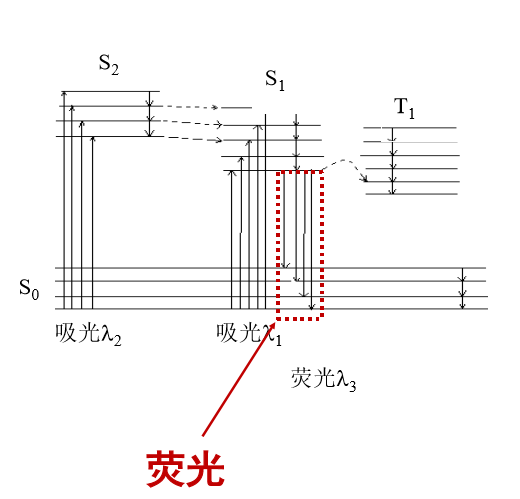
\includegraphics[width=10cm]{chp4_flu_principle}
	\label{fig:chp4fluprinciple}
	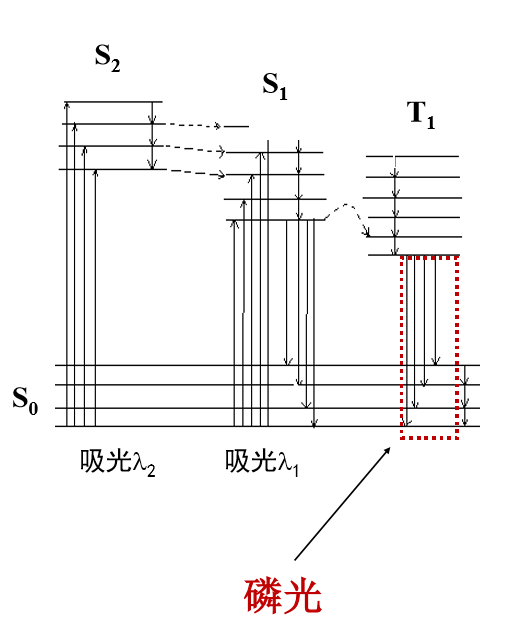
\includegraphics[width=10cm]{chp4_phos_principle}
	\label{fig:chp4phosprinciple}
	\caption{}
\end{figure}



\section{荧光定量分析基础}
\subsection{荧光量子产率}

\begin{definition*}{荧光量子产率$\Phi$}{}
	 表示物质发射荧光的能力,如果一个分子将吸收的光子全部释放,则其量子产率为$100\%$。
	\begin{equation*}
		\Phi =\frac{\text{发射荧光的分子数}}{\text{激发态的分子数}}=\frac{\text{发射的光子数}}{\text{吸收的光子数}}
	\end{equation*}
\end{definition*}

$\phi$与失活过程的速率常数k有关:
\begin{equation}
	\Phi =\frac{k_{f}}{k_{f}+k_{i}+k_{ec}+k_{ic}}
\end{equation}
\begin{note}
	\begin{itemize}
		\item $k_{f}$:荧光辐射速率
		\item $k_{i}$:系间跨越速率,重原子存在下$k_{i}$较大
		\item $k_{ec}$:外转换速率
		\item $k_{ic}$:内转换速率
		\begin{itemize}
			\item 分子碰撞几率越大,$k_{ec}$与$k_{ic}$越大。
		\end{itemize}
	\end{itemize}
\end{note}
凡是使荧光速率常数$k_{f}$增大而使其他失活过程(系间窜越、 外转换、内转换)的速率常数减小的因素都可使荧光增强。

\subsection{荧光与分子结构的关系}
\subsubsection{跃迁类型}
$\pi^{\star} \rightarrow \pi$的荧光效率高,系间跨越过程的速率常数小,有利于荧光的产生,故发射 $\pi^{\star} \rightarrow \pi$跃迁比$\pi^{\star} \rightarrow n$跃迁更常见;

\subsubsection{共轭效应}
提高共轭度有利于增加荧光效率并产生红移;
\begin{itemize}
	\item 芳香族化合物的荧光最常见且最强,大多数未取代芳烃在溶液中发荧光,随着环的数目和共轭度增加,荧光峰红移,$\phi \uparrow$。简单杂环化合物不发荧光,但具有稠环结构的杂环化合物都发荧光;
	\item 任何有利于提高$\pi$电子共轭度的结构改变,都将提高荧光量子产率,或使荧光波长向长波长方向移动;
	\item 电子共轭程度越大,越容易产生荧光;环越大,发光峰红移程度越大,发光往往越强;
	\item 共轭环数相同的芳香族化合物,线性环结构的荧 光波长比非线性者要长。
\end{itemize}

\subsubsection{刚性平面结构}
可降低分子振动,减少与溶剂的相互作用,故具有很强的荧光;
\begin{itemize}
	\item 试剂与金属形成配合物后,刚性增强,荧光也增强;
	\item 荧光分子在固体表面荧光强度更高;
\end{itemize}
\subsubsection{取代基效应}
\begin{itemize}
	\item 芳环上有羧基、羰基、亚硝基、巯基等吸电 子基团取代时,荧光减弱;取代基的n电子云并不与芳环上$\pi$电子云共平面;
	\item 给电子取代基如-\ce{OH}、-\ce{NH_{2}}、-$\ce{CN}$、-$\ce{CH_{3}}$等会使荧光强度增加;取代基上的n电子的电子云几乎和芳环上的π轨道平行, 因而共享了共轭$\pi$电子结构,产生了p- $\pi$共轭效应,扩大了共轭双键体系。
	\item 重原子效应: 含有重原子的分子中,使系间窜跃的几率大,荧光强度随 卤素相对原子质量的增强而减弱,磷光增强。如:Br,I;
	\item 取代基的位置:
	\begin{itemize}
		\item 对位、邻位取代增强荧光,间位取代抑制荧光;
		\item 双取代或多取代基的影响较难预测;
		\item 取代基之间能形成氢键增加分子的平面性,荧光增强;
		\item 两种性质和作用不同的取代基共存时,其中一个起主导作用。
	\end{itemize}
\end{itemize}

\subsection{荧光定量分析基础}
荧光物质浓度很稀时,所发射的荧光相对强度$I_{f}$可用下式表示:
\begin{theorem*}{荧光强度表达式}
	\begin{equation*}
		I_{f}=K'\Phi_{f}I_{0}(1-e^{-A})
	\end{equation*}
\end{theorem*}
随着荧光物质浓度增加,吸光度A增加,相对荧光强度增加。
\begin{itemize}
	\item 当溶液很稀,吸光度A<0.05时,$e^{-A}\approx 1-A$,则$I_{f}=K_{c}$,在一定条件下,用𝐼0一定的入射光激发荧光溶液时,其发射的荧光强度与荧光物质的浓度成正比。
	\item 当溶液的A≥0.05时将产生浓度效应,使荧光强度与浓度的关系偏离线性。
\end{itemize}
\begin{figure}
	\centering
	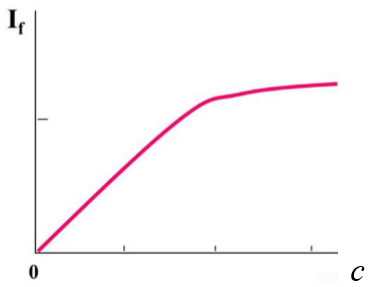
\includegraphics[width=5 cm]{chp4_conse_eff.png}
	\label{fig:chp4conseeff}
	\caption{荧光定量吸收的浓度效应}
\end{figure}
\subsubsection{荧光猝灭}
\begin{definition*}{荧光猝灭}
	荧光分子与溶剂或其他物质分子作用使荧光强度减弱的现象叫荧光猝灭,能使荧光强度降低的物质称为荧光猝灭剂。
\end{definition*}
猝灭种类:
\begin{itemize}
	\item 自猝灭:荧光物质浓度较大时,会使荧光强度降低。
	\begin{itemize}
		\item 荧光物质分子之间的碰撞能量损失:单重激发态的分子在发生荧光之前和未激发的荧光物质分子碰撞。
		\item 荧光物质的自吸收;
		\item 荧光物质分子的缔合:二聚体或多聚体。
	\end{itemize}
	\item 电荷转移猝灭:激发态分子比基态具有更强的与其他物质发生氧化还原反应的能力,从而导致荧光猝灭,这种现象称为电荷转移猝灭,如:
	
	甲基蓝分子$M*+\ce{Fe^{2+}} \rightarrow M^{-}+\ce{Fe^{3+}}$;
	\item 转入三线态的淬灭:含溴化物、碘化物、硝基化合物、重氮化合物、 羰基化合物及某些杂环化合物容易转变为三重态,因而易使荧光淬灭;
\end{itemize}

\section{荧光分光光度计}
基本组成: 
\begin{figure}[ht]
	\centering
	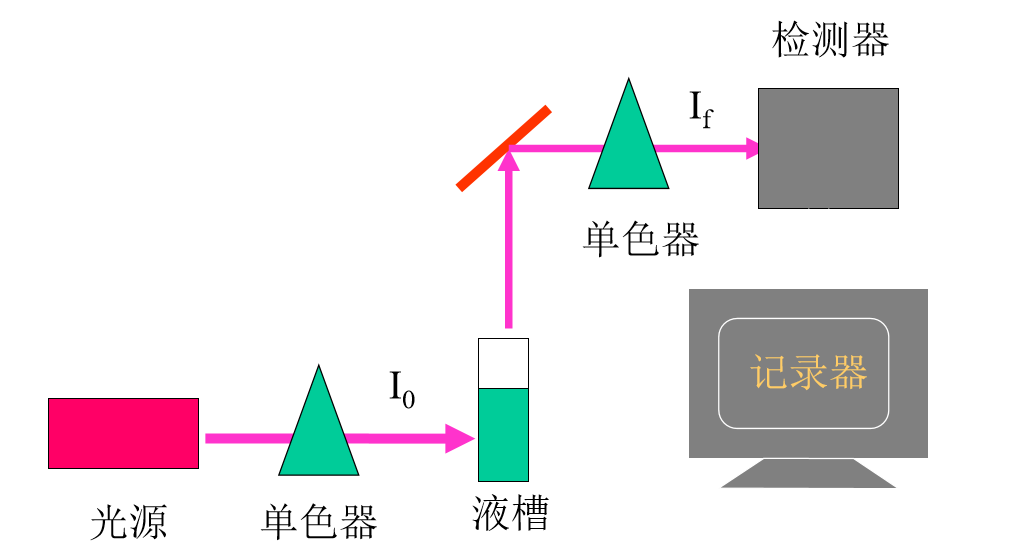
\includegraphics[width=0.7\linewidth]{chp4_instru.png}
	\label{fig:chp4instru}
	\caption{荧光分光光度计}
\end{figure}
\begin{itemize}
	\item 光源
	\begin{itemize}
		\item 高压汞灯,平均寿命1500-3000 h,发射365,405,436 nm作为激发光;
		\item 氙灯,寿命2000 h,发射250-800 nm的连续光谱;
		\item 激光,发光强度大,能极大地提高荧光分析的灵敏度。
	\end{itemize}
	\item 单色器:常用光栅
	\begin{itemize}
		\item 第一单色器选激发光波长,第二单色器选荧光波长
		\item 灵敏度较高,波长范围较宽,能扫描光谱
		\item 主要缺点:杂散光较大,有不同级次的谱线干扰
	\end{itemize}
	\item 试样室:固体样品使用固体试样架,液体样品使用四面透光的石英池
	\item 光电倍增管(PMT):较高级仪器采用光电二极管阵列检测器(PDA),它具有检测效率高、线性响应好、坚固耐用和寿命长等优点,最主要的优点是扫描速度快,可同时记录下完整的荧光光谱(即三维光谱)
	\item 读出装置:记录仪、阴极示波器、显示器等。记录仪用于扫描光谱,阴记示波器的显示速度比记录仪更快。
\end{itemize}

\begin{note}
	和紫外-可见吸收光谱相比较,荧光为什么灵敏度较高?

	因为荧光分析的荧光和入射光之间成直角,而不在一条直线上,所以是在黑背景下检测荧光;而分光光度法的接收器与入射光在一条直线上,所以它是在亮背景下检测的,当试样浓度很低时,吸收微弱,分光光度法的$I$与$I_{0}$非常接近,在这种情况下,让仪器检测一组衬比度较低的信号是十分困难的,因此荧光分析法比分光光谱法灵敏度高。
\end{note}




\end{document}
